\documentclass[stu, 12pt, donotrepeattitle, floatsintext, longtable]{apa7}

\usepackage[spanish,es-tabla]{babel}
\usepackage[utf8]{inputenc}
\usepackage[T1]{fontenc}

% --- Tipografia APA 7 --------------------------------------------------
% La clase apa7 ya cumple por defecto con margenes de 1 pulgada,
% interlineado doble y los 5 niveles de encabezado (centrado/negrita,
% izquierda/negrita, izquierda/negrita-cursiva, etc.) segun su propia
% documentacion. La 7ma edicion de APA acepta tanto fuentes serif de
% 12pt (Times New Roman) como Computer Modern 10pt (la fuente por
% defecto de LaTeX), asi que no es obligatorio cambiar la fuente. Se
% fuerza aqui Times (via mathptmx) para que el PDF final se vea
% consistente con "Times New Roman 12pt", que es el estandar mas
% reconocible y el que suele pedirse en cursos que no aceptan LaTeX.
\usepackage{mathptmx}

\usepackage{graphicx}
\usepackage{svg}

\usepackage{listings}
\usepackage{xcolor}

\lstdefinestyle{pseudocodigo}{
    basicstyle=\ttfamily\small,
    breaklines=true,
    frame=single,
    numbers=left,
    numberstyle=\tiny,
    columns=fullflexible,
    keepspaces=true
}

\usepackage{longtable}
\usepackage{booktabs}

\usepackage{hyperref}
\hypersetup{
    colorlinks=true,
    linkcolor=black,
    citecolor=black,
    urlcolor=blue
}

\usepackage[style=apa, backend=biber]{biblatex}
\DeclareLanguageMapping{spanish}{spanish-apa}
\addbibresource{referencias.bib}

% Logo institucional en el header de cada pagina (esquina superior derecha).
\IfFileExists{assets/logo-una.png}{%
    \fancyhead[R]{\includegraphics[height=1cm]{assets/logo-una.png}}%
}{}%

% Punto centralizado para overrides de encabezados (h1-h5)
% Configuracion centralizada de niveles de encabezado (h1-h5).
%
% apa7.cls YA formatea \section, \subsection, \subsubsection, \paragraph
% y \subparagraph segun las reglas de APA 7 de forma nativa y correcta:
%   h1 \section       -> centrado, negrita, mayus/minus
%   h2 \subsection    -> alineado izquierda, negrita, mayus/minus
%   h3 \subsubsection -> alineado izquierda, negrita cursiva, mayus/minus
%   h4 \paragraph     -> con sangria, negrita, termina en punto, texto sigue en la misma linea
%   h5 \subparagraph  -> con sangria, negrita cursiva, termina en punto, texto sigue en la misma linea
%
% NO tocar el formato de estos comandos con paquetes como titlesec: eso
% pisaria el comportamiento nativo de apa7.cls, que ya es compliant con el
% manual oficial (ver informe/formato.tex para el resto de paquetes usados).
%
% Si en el futuro hace falta AJUSTAR algo puntual (espaciado extra entre
% secciones, tamano de fuente especifico, etc.), centralizar esos cambios
% aqui usando \titlespacing o redefiniendo el comando puntual, en vez de
% hacerlo directo en cada archivo de seccion. Este archivo esta vacio por
% ahora a proposito: el formato nativo de apa7.cls no requiere overrides.



\title{
    Investigación \#1: Caso de Estudio\\
    Diseño e Implementación del Sistema de Gestión Académica de la Universidad XUNA
}
\author{\textbf{Estudiantes:} \\ Joanfer Hidalgo Chaves \\ Santiago Hernández Chaves \\ Justin Angulo Artavia}
\affiliation{Escuela de Informática, Universidad Nacional de Costa Rica}
\course{EIF207, Estructuras de Datos}
\professor{\textbf{Docente:} \\ Msc. Johnny Villalobos Murillo}
\note{II Ciclo 2026}
\duedate{\today}

\begin{document}
\maketitle
\clearpage

\tableofcontents
\newpage

% !TEX root = ../main.tex
\section{Introducción}

En la actualidad, las organizaciones manejan grandes cantidades de
información que deben mantenerse organizadas para facilitar su consulta,
actualización, almacenamiento y recuperación. En instituciones como las
universidades, esta necesidad adquiere especial importancia debido al
volumen de datos personales y académicos que deben administrarse de forma
constante.

Antes de desarrollar un sistema informático es necesario comprender el
problema que se desea resolver, identificar los datos que serán
administrados y definir estructuras adecuadas para representarlos. De
igual forma, se debe considerar la eficiencia de las operaciones que se
realizarán sobre dicha información, debido a que distintas soluciones
pueden requerir diferentes cantidades de tiempo y recursos.

La presente investigación analiza el caso de la Universidad XUNA, una
institución con aproximadamente 25\,000 estudiantes que busca reemplazar
el uso de formularios impresos, hojas electrónicas y programas
independientes por un Sistema de Gestión Académica centralizado. El
sistema deberá permitir administrar información personal y académica de
los estudiantes, además de realizar operaciones como registrar, buscar,
modificar, consultar y generar reportes.

A partir de este caso se estudiarán conceptos fundamentales relacionados
con las estructuras de datos, entre ellos el dato, los Tipos de Datos
Abstractos, los registros, los arreglos, las funciones, el costo
computacional y los mecanismos de almacenamiento mediante archivos
secuenciales e indexados. El objetivo es establecer una propuesta de
diseño organizada y técnicamente justificada que sirva como base para el
posterior desarrollo del sistema.
\newpage
% !TEX root = ../main.tex
\section{Análisis del problema}
% TODO: resumen del caso XUNA y las restricciones técnicas del enunciado.

\subsection{Restricciones técnicas del proyecto}
% TODO: C++ estructurado, sin POO, sin STL, structs, fopen/fread/fwrite/fseek.

\subsection{Preguntas arquitectónicas planteadas}
% TODO: desarrollar en prosa cada pregunta, citando por qué se descartó cada alternativa.
% Ver docs/decisiones/ para el razonamiento ya resuelto.
%
% - ¿Cómo representar los datos sin POO ni STL?
% - ¿Cómo evitar cargar todo el volumen en RAM a medida que crece?
% - ¿Cómo buscar por varias llaves sin árboles?
% - ¿Cómo evitar que cada inserción cueste O(n)?
% - ¿Cómo persistir la información entre ejecuciones?

\newpage
% !TEX root = ../main.tex
\section{Identificación de los datos presentes en el caso}
% TODO: listar los catorce datos que pide la Oficina de Registro.

\newpage
% !TEX root = ../main.tex
\section{Clasificación de los datos según su Tipo de Dato Abstracto}

Una vez identificados los datos que forman parte del expediente de cada
estudiante, es necesario determinar la naturaleza de la información que
representa cada uno. Esta clasificación permite definir posteriormente
la forma en que los datos serán almacenados y manipulados dentro del
programa.

Para este diseño se consideran tipos como entero, real, cadena de
caracteres, dato enumerado y fecha. La clasificación lógica de cada dato
se presenta en la siguiente tabla.

\begin{longtable}{p{3.8cm} p{3.2cm} p{7cm}}
\toprule
Dato & Tipo de dato & Justificación \\
\midrule
\endhead

Número de carné &
Entero &
Representa el identificador numérico asignado por la universidad a cada
estudiante. Se utilizará principalmente como llave de búsqueda y
referencia del registro. \\

Número de identificación &
Cadena de caracteres &
Aunque está compuesto principalmente por dígitos, funciona como un
identificador y puede variar en longitud o incluir caracteres según el
tipo de documento. Por esta razón se trata como información textual. \\

Nombre &
Cadena de caracteres &
Está compuesto por una secuencia de caracteres alfabéticos y forma parte
de la información personal del estudiante. \\

Apellidos &
Cadena de caracteres &
Corresponde a información textual. En el diseño posterior podrá
separarse en diferentes campos para facilitar búsquedas y ordenamientos. \\

Fecha de nacimiento &
Fecha &
Está formada por varios valores relacionados entre sí, específicamente
día, mes y año. Por esta razón resulta conveniente representarla mediante
un tipo compuesto destinado al manejo de fechas. \\

Sexo &
Enumerado &
Corresponde a un conjunto limitado de valores posibles, por lo que puede
representarse mediante un dominio cerrado en lugar de utilizar texto
libre. \\

Carrera &
Entero de referencia &
Puede almacenarse mediante un código numérico que identifique una carrera
dentro de un catálogo, evitando repetir el nombre completo de la carrera
en cada registro. \\

Nivel académico &
Enumerado &
Representa una categoría dentro de un conjunto limitado de niveles
académicos definidos por el sistema. \\

Correo electrónico &
Cadena de caracteres &
Puede contener letras, números y símbolos, por lo que debe almacenarse
como una secuencia de caracteres. \\

Número telefónico &
Cadena de caracteres &
Aunque contiene dígitos, no representa una cantidad sobre la cual deban
realizarse operaciones matemáticas. Se utiliza únicamente como dato de
contacto. \\

Dirección &
Cadena de caracteres &
Contiene texto de longitud variable que puede incluir letras, números,
espacios y otros caracteres. \\

Cantidad de créditos aprobados &
Entero &
Representa una cantidad discreta de créditos acumulados por el estudiante
y puede utilizarse en operaciones de comparación y actualización. \\

Promedio general &
Real &
Puede contener una parte decimal, por lo que requiere un tipo numérico
capaz de representar valores fraccionarios. \\

Estado del estudiante &
Enumerado &
Representa un conjunto limitado de condiciones posibles del estudiante,
como activo o inactivo. \\

\bottomrule
\end{longtable}

Esta clasificación distingue entre los datos que representan cantidades
numéricas y aquellos que, aunque puedan contener dígitos, funcionan
únicamente como identificadores. Por ejemplo, el número telefónico y el
número de identificación no se utilizan para realizar cálculos, mientras
que la cantidad de créditos aprobados y el promedio general sí forman
parte de operaciones académicas.

También se identifican datos cuyo dominio está limitado a un conjunto
determinado de valores, como el sexo, el nivel académico y el estado del
estudiante. Estos pueden tratarse como tipos enumerados para evitar el
almacenamiento de valores arbitrarios.

La clasificación anterior establece la representación lógica de los
datos. En las siguientes secciones estos tipos se traducen a estructuras
concretas del lenguaje C++, respetando las restricciones del proyecto y
las necesidades de almacenamiento del sistema.
\newpage
% !TEX root = ../main.tex
\section{Diseño del registro Estudiante}

El enunciado de la investigación pide administrar trece datos por
estudiante: número de carné, identificación, nombre, apellidos, fecha de
nacimiento, sexo, carrera, nivel académico, correo electrónico, número
telefónico, dirección, cantidad de créditos aprobados y promedio general,
además del estado del estudiante. El enunciado no propone ninguna forma de
organizar estos datos, solo los enumera como requisitos que el sistema
debe guardar.

El primer intento del equipo fue juntar los trece campos en un único
registro. Al revisarlo con cuidado apareció un problema: esos trece campos
no cambian con la misma frecuencia ni se usan juntos en las mismas
operaciones. El nombre y la fecha de nacimiento de un estudiante casi
nunca cambian una vez matriculado. El promedio y los créditos aprobados se
actualizan varias veces durante la carrera del estudiante, cada período
lectivo. El correo, el teléfono y la dirección se consultan juntos
normalmente solo cuando hace falta contactar al estudiante, y casi nunca
al mismo tiempo que se actualiza el promedio.

Juntar estos tres grupos en un solo registro significa que actualizar el
promedio de un estudiante, algo que ocurre constantemente, obliga también
a leer y reescribir su nombre, su fecha de nacimiento, su correo y su
dirección, aunque ninguno de esos datos haya cambiado.

Por esa razón se decidió dividir el registro en tres structs
independientes, cada uno guardado en su propio archivo binario
(\texttt{identidad.dat}, \texttt{academico.dat}, \texttt{contacto.dat}).
El criterio de separación es la frecuencia y el patrón de uso de cada
grupo de campos, no una división arbitraria. Esta técnica se conoce como
particionamiento vertical y es la misma que aplican los motores de bases
de datos relacionales cuando separan columnas de una entidad lógica en
tablas físicas distintas por razones de rendimiento.

Los tres structs se mantienen alineados por posición: el registro en la
posición $i$ de \texttt{identidad.dat} corresponde al mismo estudiante que
el registro en la posición $i$ de \texttt{academico.dat} y de
\texttt{contacto.dat}. Gracias a esto, un único índice (carné apuntando a
posición) basta para ubicar al estudiante en cualquiera de los tres
archivos, sin necesidad de tres índices repetidos.

\subsection{IdentidadEstudiante}
Datos que identifican al estudiante como persona: carné, identificación,
nombre, apellidos, fecha de nacimiento y sexo.

\begin{lstlisting}[style=pseudocodigo]
typedef struct {
    int carne;
    char identificacion[13];
    TipoIdentificacion tipoIdentificacion;
    char nombre[21];
    char apellido1[21];
    char apellido2[21];
    Fecha fechaNacimiento;
    int sexo;
} IdentidadEstudiante;
\end{lstlisting}

\subsection{AcademicoEstudiante}
Datos de la situación académica actual del estudiante, que cambian cada
período lectivo.

\begin{lstlisting}[style=pseudocodigo]
typedef struct {
    int carne;
    int carrera;
    int nivelAcademico;
    int creditosAprobados;
    float promedio;
    int estado;
} AcademicoEstudiante;
\end{lstlisting}

\subsection{ContactoEstudiante}
Datos usados para comunicarse con el estudiante, que cambian con poca
frecuencia.

\begin{lstlisting}[style=pseudocodigo]
typedef struct {
    int carne;
    char correo[41];
    char telefono[9];
    char direccion[81];
} ContactoEstudiante;
\end{lstlisting}

\newpage
% !TEX root = ../main.tex
\section{Justificación de cada uno de los campos del registro}

Todos los campos de tipo texto se implementan como \texttt{char[]} de
tamaño fijo, nunca como cadenas dinámicas, porque el tamaño fijo es lo que
permite calcular el \texttt{offset} de cualquier registro dentro de su
archivo mediante \texttt{posición} $\times$ \texttt{sizeof(struct)}.

Cada arreglo de caracteres reserva un byte adicional para el carácter nulo
(\texttt{'\textbackslash 0'}), que en C marca el final real de la cadena:
funciones como \texttt{strlen}, \texttt{strcmp} o
\texttt{printf("\%s", \ldots)} no conocen la longitud de una cadena de
antemano, y sin ese byte seguirían leyendo memoria más allá del dato
válido.

\begin{longtable}{p{2.7cm} p{2.2cm} p{1.5cm} p{6.5cm}}
\toprule
Campo & Tipo & Tamaño & Justificación \\
\midrule
\endhead

carne &
int &
4 B &
Llave primaria numérica, requerida explícitamente por el caso de estudio
junto con la identificación como campo de búsqueda independiente. \\

identificacion &
char[13] &
13 B &
Cubre el caso más ancho entre cédula física (9 dígitos), DIMEX de
residencia (entre 11 y 12 dígitos) y pasaporte alfanumérico: 12 caracteres
más el terminador nulo. \\

tipoIdentificacion &
enum (int) &
4 B &
Distingue nacional/DIMEX/pasaporte sin mezclar esa información dentro del
campo de texto. \\

nombre &
char[21] &
21 B &
20 caracteres útiles, margen razonable para nombres compuestos. \\

apellido1, apellido2 &
char[21] c/u &
42 B &
Separados en vez de un solo campo \texttt{apellidos}, para permitir
búsquedas y ordenamientos por apellido de forma consistente. \\

fechaNacimiento &
struct Fecha &
12 B &
TAD propio (día, mes, año como \texttt{int}), reutilizable y con sus
propias reglas de validez. \\

sexo &
enum (int) &
4 B &
Dominio cerrado, representado como entero en vez de texto libre. \\

carrera &
int &
4 B &
Referencia a un catálogo de carreras en vez de repetir el nombre completo
en cada registro. \\

nivelAcademico &
enum (int) &
4 B &
Dominio cerrado (pregrado, grado, posgrado, etc.). \\

creditosAprobados &
int &
4 B &
Cantidad entera, sin componente fraccionario. \\

promedio &
float &
4 B &
Requiere parte decimal. \\

estado &
int (bool a mano) &
4 B &
0 para inactivo, 1 para activo; sostiene el borrado lógico sin usar
\texttt{bool} de C++. \\

correo &
char[41] &
41 B &
Margen suficiente para direcciones institucionales y personales comunes. \\

telefono &
char[9] &
9 B &
8 dígitos (formato costarricense) más el terminador nulo. \\

direccion &
char[81] &
81 B &
Texto libre de longitud variable, con un tope generoso fijo. \\

\bottomrule
\end{longtable}

\newpage
% !TEX root = ../main.tex
\section{Diseño del arreglo que almacenará los estudiantes}

El arreglo de registros completos no se carga en memoria principal: vive
en disco, en los tres archivos binarios descritos en la sección anterior.
Lo que sí reside en RAM en todo momento es un arreglo mucho más liviano,
al que llamamos \textbf{mapa de posiciones}: guarda únicamente la llave de
búsqueda, la posición física del registro en disco y su estado, sin el
resto de los datos del estudiante (el funcionamiento completo de este
mapa se detalla en la sección de archivo indexado).

\subsection{Por qué cargar todo en memoria no escala}

\begin{longtable}{p{4.5cm} p{3cm} p{3cm} p{2cm}}
\toprule
Cantidad de estudiantes & Registro completo (3 archivos) & Solo mapas de posiciones (3 mapas) & Ahorro \\
\midrule
\endhead
25\,000 & $\approx$ 6.2 MB & $\approx$ 1.2 MB & 5 veces \\
100\,000 & $\approx$ 25 MB & $\approx$ 4.8 MB & 5 veces \\
1\,000\,000 & $\approx$ 259 MB & $\approx$ 48 MB & 5 veces \\
\bottomrule
\end{longtable}

El cálculo usa 259 bytes por estudiante (suma de los tres structs de la
sección de diseño del registro, sin contar relleno de alineación) contra
16 bytes por entrada de mapa (carné, posición y estado), multiplicado por
tres mapas (por carné, por identificación, por apellido). Aunque un
millón de registros completos (aproximadamente 259 MB) todavía cabría en
la memoria de una máquina moderna, el diseño no depende de esa suposición:
el costo en RAM de los mapas crece mucho más lento que el de los datos
completos, por lo que la arquitectura sigue siendo viable sin importar
cuánto crezca la matrícula de la universidad.

\newpage
\section{Representación gráfica del arreglo}

La arquitectura de este arreglo se explica en las secciones~\ref{sec:diseno-arreglo} y~\ref{sec:archivo-indexado}; 
para evitar redundancia en esta seccion no se explicara la justificacion aun.

\begin{figure}[h]
    \centering
    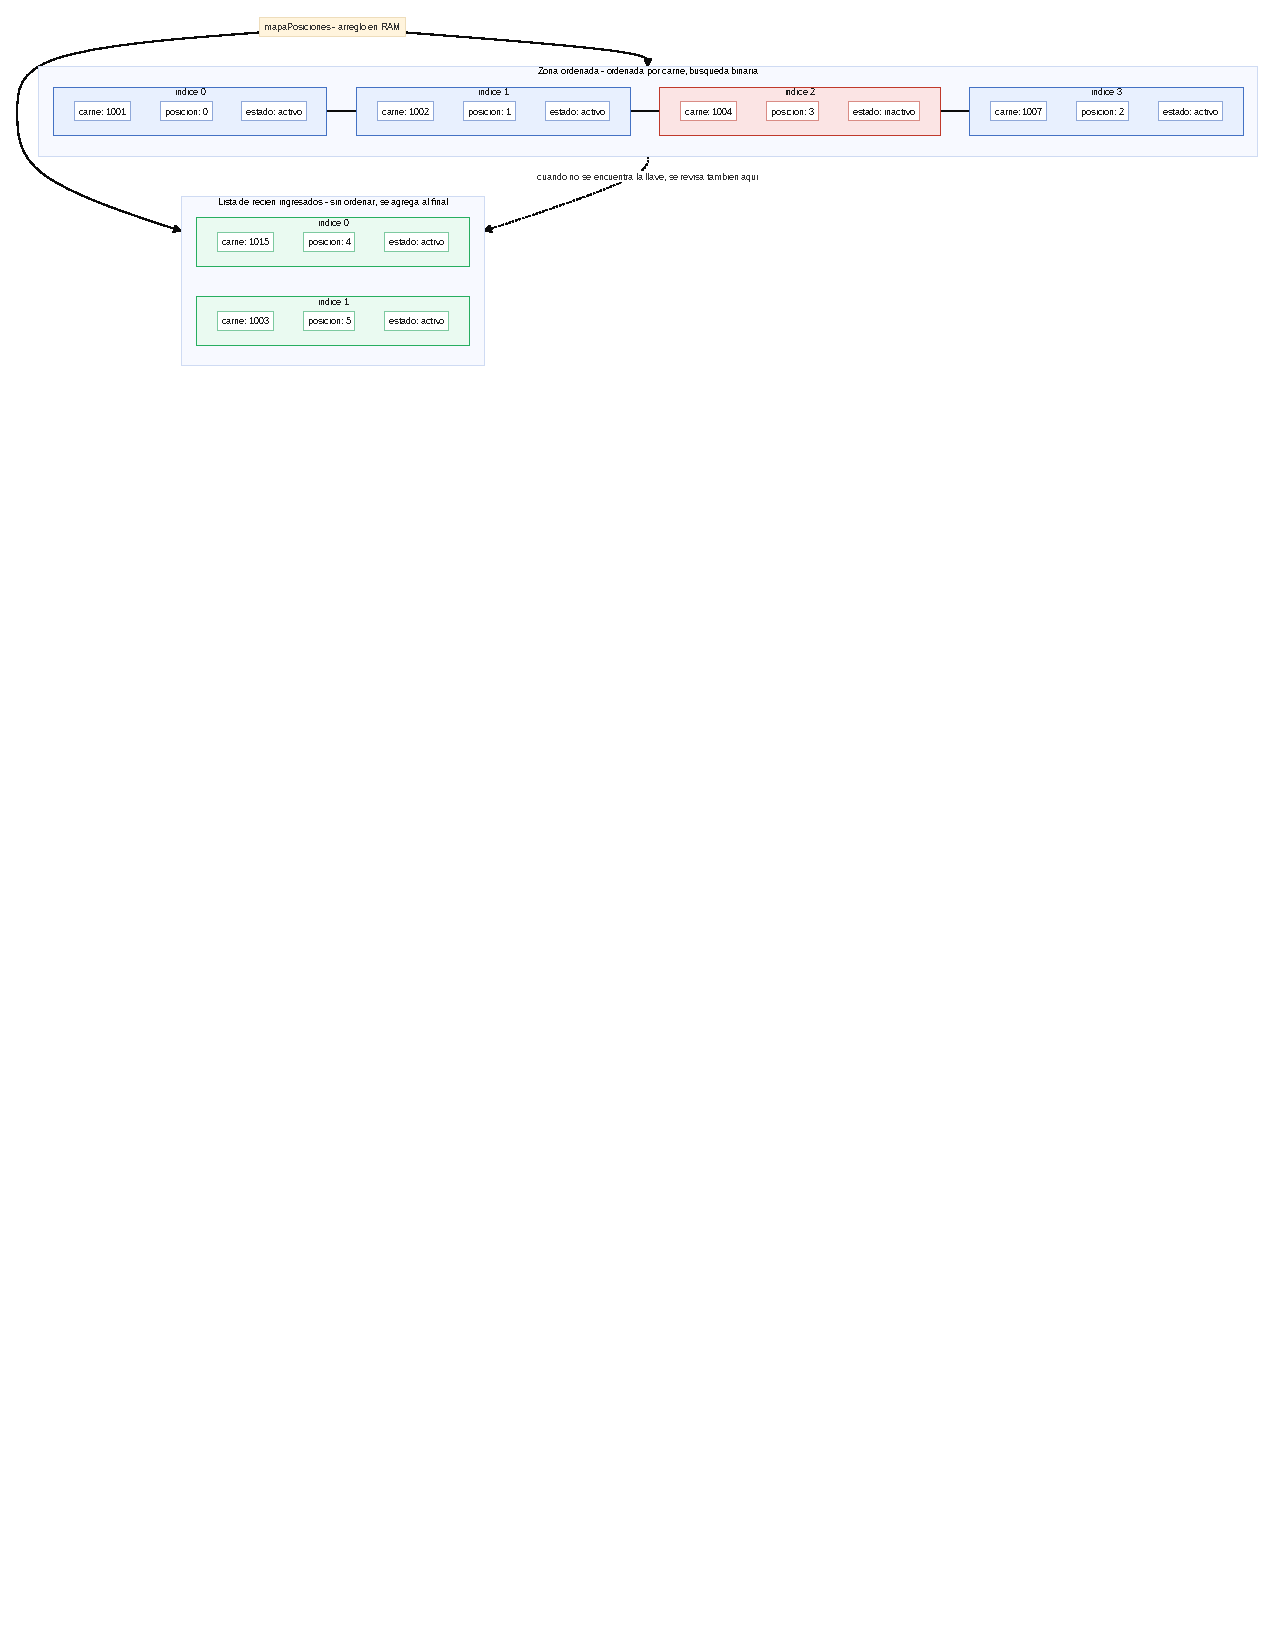
\includegraphics[width=0.85\textwidth]{../diagramas/output/mapa-posiciones-ram.pdf}
    \caption{El mapa de posiciones como arreglo en RAM}
    \label{fig:mapa-posiciones-ram}
\end{figure}

La figura~\ref{fig:mapa-posiciones-ram} muestra las dos zonas del mapa por carné descritas en la subsección~\ref{sec:mapa-por-carne} 
aparecen como dos arreglos separados: 
\begin{enumerate}
    \item La \textbf{zona ordenada} (índices 0 a 3)
    \item La \textbf{lista de recién ingresados} (índice 0, con el carné 1015 que todavía no fue integrado)
\end{enumerate}

Cada celda, en cualquiera de las dos zonas, tiene la misma composición de tres campos justificada en la subsección~\ref{sec:composicion-entrada}. 
La celda en rojo (carné 1004) es el mismo ejemplo de estado inactivo usado en la sección~\ref{sec:archivo-indexado}.

\newpage

\begin{figure}[h]
    \centering
    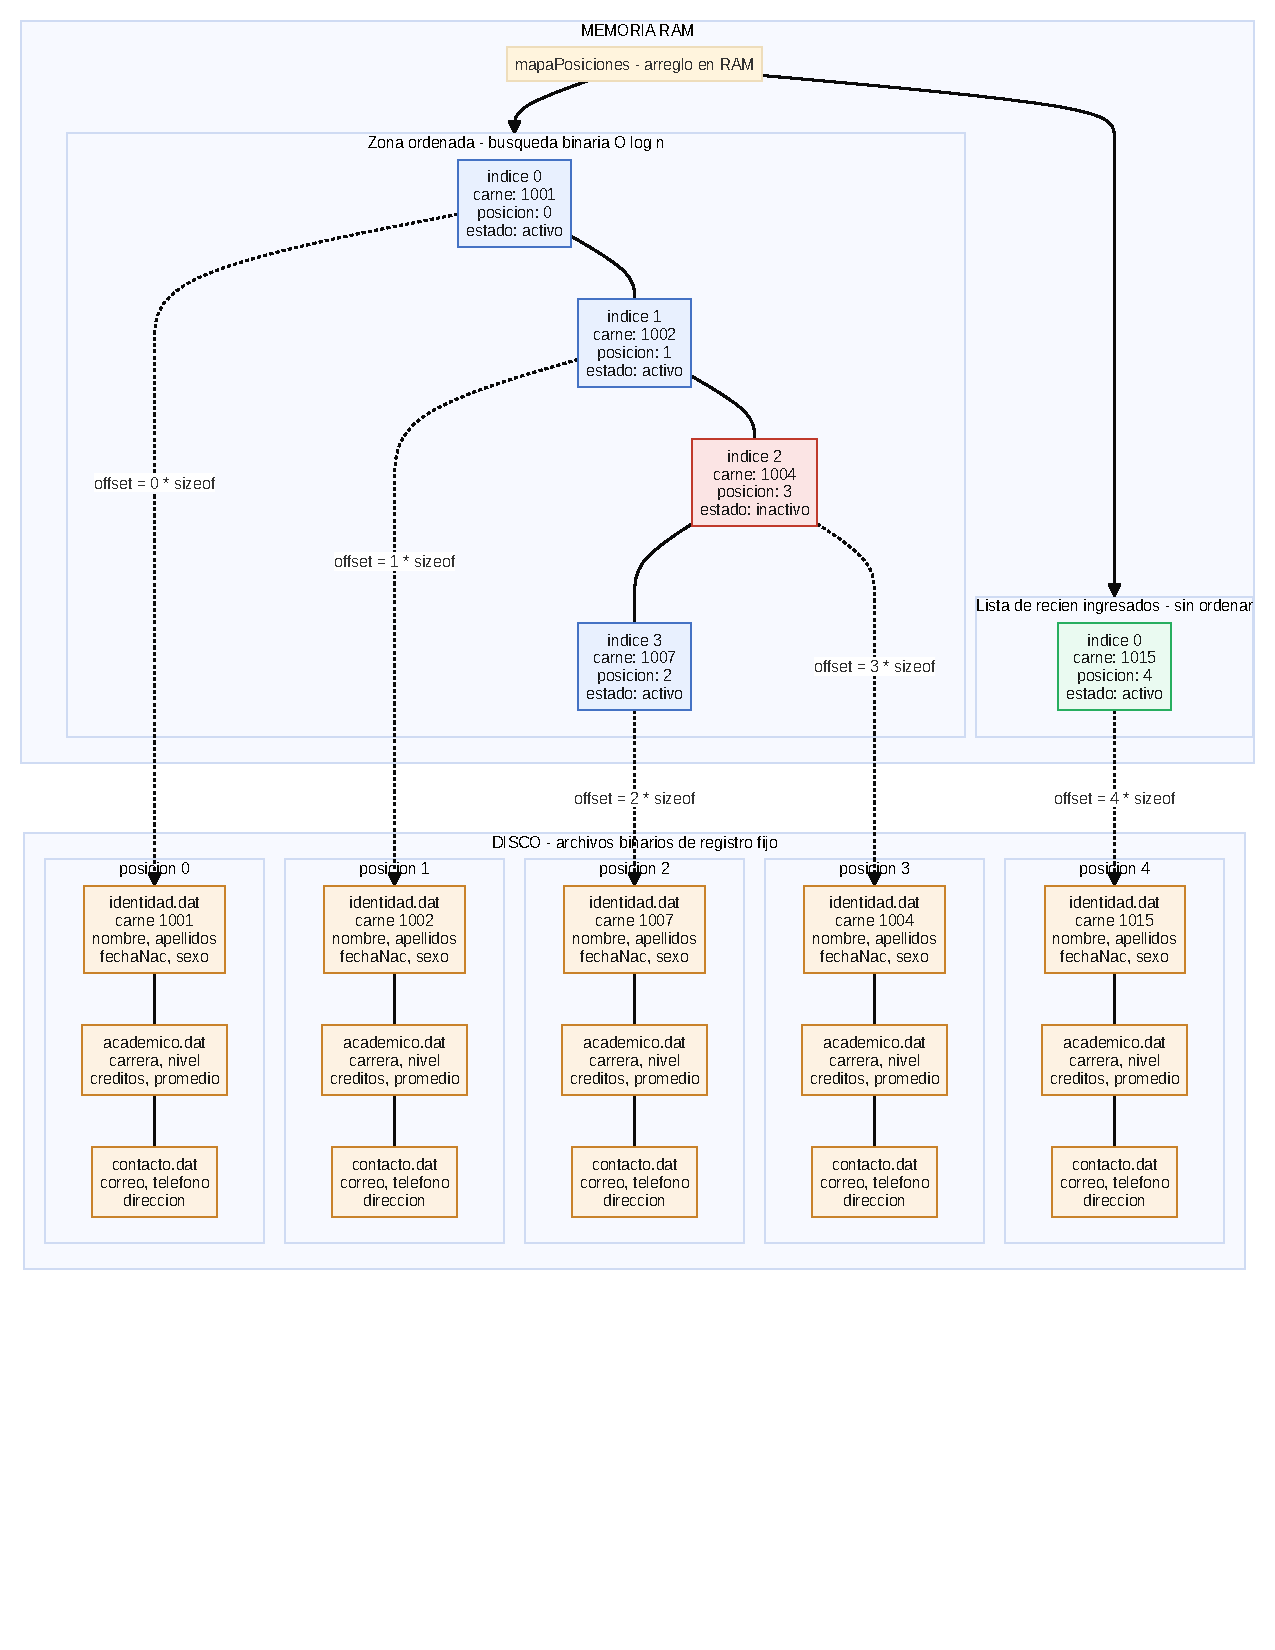
\includegraphics[width=0.95\textwidth]{../diagramas/output/arreglo-estudiantes.pdf}
    \caption{Relación entre el mapa de posiciones en RAM y los archivos en disco}
    \label{fig:arreglo-estudiantes}
\end{figure}

La figura~\ref{fig:arreglo-estudiantes} agrega los tres archivos en disco (sección~\ref{sec:archivo-secuencial}) a la misma estructura de la
figura anterior. Las flechas punteadas son el cálculo de \texttt{offset} de la sección~\ref{sec:archivo-secuencial} aplicado a
cada entrada del mapa: 
\begin{itemize}
    \item El carné 1007 (zona ordenada, índice 3) apunta a la posición 2 en disco
    \item El carné 1004 (inactivo) apunta a la posición 3
    \item El carné 1015 (lista de recién ingresados) apunta a la posición 4, la más reciente
\end{itemize}

Las tres columnas de cada posición (\texttt{identidad.dat}, \texttt{academico.dat}, \texttt{contacto.dat}) ilustran que comparten 
índice sin necesitar una llave adicional entre ellas, también justificado en la sección~\ref{sec:archivo-secuencial}.

\newpage
% !TEX root = ../main.tex
\section{Identificación de todas las funciones necesarias}

\subsection{Módulo archivo (persistencia)}
\begin{longtable}{F{7.2cm} p{7.8cm}}
\toprule
\multicolumn{1}{p{7.2cm}}{Función} & Entrada $\rightarrow$ Salida \\
\midrule
\endhead
abrirArchivo(nombre, modo) &
    nombre, modo $\rightarrow$ FILE* \\
cerrarArchivo(fp) &
    FILE* $\rightarrow$ void \\
calcularOffset(posicion, tamRegistro) &
    posición, tamaño $\rightarrow$ offset en bytes \\
leerRegistroEnOffset(fp, offset, destino) &
    offset $\rightarrow$ registro leído \\
escribirRegistroEnOffset(fp, offset, registro) &
    offset, registro $\rightarrow$ éxito o error \\
agregarRegistroAlFinal(fp, registro) &
    registro $\rightarrow$ offset asignado \\
contarRegistros(fp, tamRegistro) &
    sin entrada $\rightarrow$ cantidad total \\
\bottomrule
\end{longtable}


\subsection{Módulo de mapas de posiciones (RAM)}

\begin{longtable}{p{7.2cm} p{7.8cm}}
\toprule
Función & Entrada $\rightarrow$ Salida \\
\midrule
\endhead
cargarMapaDePosiciones() &
    sin entrada $\rightarrow$ mapa cargado desde disco \\
buscarPosicionPorCarne(carne) &
    carné $\rightarrow$ posición o "no encontrado" \\
registrarPosicionEnMapa(carne, posicion) &
    carné, posición $\rightarrow$ éxito \\
fusionarRecienIngresados() &
    sin entrada $\rightarrow$ mapa con zona ordenada y lista de recién ingresados fusionadas \\
marcarInactivoEnMapa(carne) &
    carné $\rightarrow$ éxito \\
construirMapaPorCampo(campo) &
    campo $\rightarrow$ mapa ordenado por ese campo \\
buscarPosicionesPorCampo(campo, valor) &
    valor $\rightarrow$ lista de posiciones \\
guardarMapasEnDisco() &
    sin entrada $\rightarrow$ mapas guardados en \texttt{.idx} \\
\bottomrule
\end{longtable}


\subsection{Módulo estudiante (lógica de negocio)}
\begin{longtable}{p{7.2cm} p{7.8cm}}
\toprule
Función & Entrada $\rightarrow$ Salida \\
\midrule
\endhead
registrarEstudiante(datos) &
    datos completos $\rightarrow$ éxito \\
buscarEstudiantePorCarne(carne) &
    carné $\rightarrow$ estudiante \\
buscarEstudiantePorIdentificacion(id) &
    identificación $\rightarrow$ estudiante \\
buscarEstudiantesPorApellido(apellido) &
    apellido $\rightarrow$ lista de estudiantes \\
modificarEstudiante(carne, nuevosDatos) &
    carné, datos $\rightarrow$ éxito \\
eliminarEstudianteLogico(carne) &
    carné $\rightarrow$ éxito \\
mostrarTodosLosEstudiantes() &
    sin entrada $\rightarrow$ recorrido completo \\
mostrarEstudiantesPorCarrera(carrera) &
    carrera $\rightarrow$ lista \\
actualizarPromedio(carne, promedio) &
    carné, valor $\rightarrow$ éxito \\
actualizarCreditosAprobados(carne, creditos) &
    carné, valor $\rightarrow$ éxito \\
consultarExpedienteCompleto(carne) &
    carné $\rightarrow$ identidad más académico más contacto \\
\bottomrule
\end{longtable}


\subsection{Módulo reportes (agregados y mantenimiento)}
\begin{longtable}{p{7.2cm} p{7.8cm}}
\toprule
Función & Entrada $\rightarrow$ Salida \\
\midrule
\endhead
calcularPromedioInstitucional() &
    sin entrada $\rightarrow$ promedio \\
encontrarMayorPromedio() &
    sin entrada $\rightarrow$ estudiante \\
encontrarMayorCreditos() &
    sin entrada $\rightarrow$ estudiante \\
generarReporteEstadistico() &
    sin entrada $\rightarrow$ resumen \\
purgarInactivos() &
    sin entrada $\rightarrow$ archivo reconstruido sin registros con estado
    en cero \\
\bottomrule
\end{longtable}


\newpage
% !TEX root = ../main.tex
\section{Descripción del propósito de cada función}

\begin{longtable}{F{5.7cm} p{9.3cm}}
\toprule
\multicolumn{1}{p{5.7cm}}{Función} & Propósito \\
\midrule
\endhead
registrarEstudiante &
    Agrega un nuevo estudiante: escribe su registro en los tres archivos y lo incorpora al mapa de posiciones. \\
buscarEstudiantePorCarne &
    Recupera el expediente (identidad, académico y contacto) a partir del carné. \\
buscarEstudiantePorIdentificacion &
    Igual que la anterior, pero usando el número de identificación como llave. \\
buscarEstudiantesPorApellido &
    Recupera todos los estudiantes que comparten un apellido dado. \\
modificarEstudiante &
    Sobrescribe los campos de un estudiante existente, sin cambiar su posición ni su carné. \\
eliminarEstudianteLogico &
    Marca a un estudiante como inactivo sin borrar físicamente su registro. \\
mostrarTodosLosEstudiantes &
    Recorre y despliega el listado completo de estudiantes activos. \\
mostrarEstudiantesPorCarrera &
    Filtra y despliega los estudiantes de una carrera específica. \\
actualizarPromedio &
    Recalcula y guarda el promedio general de un estudiante. \\
actualizarCreditosAprobados &
    Recalcula y guarda la cantidad de créditos aprobados de un estudiante. \\
consultarExpedienteCompleto &
    Reúne los tres registros (identidad, académico, contacto) de un mismo estudiante. \\
calcularPromedioInstitucional &
    Calcula el promedio general de toda la población estudiantil activa. \\
encontrarMayorPromedio &
    Ubica al estudiante con el promedio más alto. \\
encontrarMayorCreditos &
    Ubica al estudiante con más créditos aprobados. \\
generarReporteEstadistico &
    Produce un resumen agregado (totales por carrera, nivel, etc.). \\
purgarInactivos &
    Reconstruye el archivo físico eliminando de forma definitiva los registros marcados como inactivos. \\
cargarMapaDePosiciones &
    Carga o reconstruye el mapa de carné en memoria al iniciar el sistema. \\
buscarPosicionPorCarne &
    Ubica, dentro del mapa, la posición de un registro a partir de su carné. \\
registrarPosicionEnMapa &
    Agrega una nueva entrada al mapa sin reordenar la zona ordenada. \\
fusionarRecienIngresados &
    Junta la lista de recién ingresados con la zona ordenada y la deja ordenada de nuevo. \\
construirMapaPorCampo &
    Genera un mapa ordenado por un campo distinto al carné (identificación o apellido). \\
buscarPosicionesPorCampo &
    Ubica una o varias posiciones a partir de un valor de un campo secundario. \\
\bottomrule
\end{longtable}


\newpage
% !TEX root = ../main.tex
\section{Pseudocódigo de las funciones principales}

El pseudocódigo se escribe en sintaxis C simplificada: condicionales,
ciclos y llamadas a función explícitas, sin declarar tipos de bajo nivel
que no aportan a entender el algoritmo. Cada bloque corresponde a un solo
camino de decisión por línea, para que sea directo de traducir a un
diagrama de flujo (ver sección de diagramas): cada \texttt{si}, cada
ciclo y cada \texttt{retornar} es un bloque separado que corresponde a un
nodo o una decisión distinta en el diagrama.

% El pseudocodigo de cada funcion vive en su propio archivo dentro de
% informe/pseudocodigo/, editable sin tocar la prosa de esta seccion.

\subsection{registrarEstudiante(datos)}
\begin{lstlisting}[style=pseudocodigo]
funcion registrarEstudiante(datos):
    si no validarFormato(datos):
        retornar ERROR

    posicion = buscarEspacioLibre()
    si posicion == NO_HAY_ESPACIO:
        posicion = expandirVector()

    escribirRegistroEnOffset(identidad.dat, posicion, datos.identidad)
    escribirRegistroEnOffset(academico.dat, posicion, datos.academico)
    escribirRegistroEnOffset(contacto.dat, posicion, datos.contacto)

    insertarEnIndicePrimario(datos.carne, posicion)

    retornar EXITO
\end{lstlisting}


\subsection{buscarEstudiantePorCarne(carne)}
\begin{lstlisting}[style=pseudocodigo]
funcion buscarEstudiantePorCarne(carne):
    posicion = buscarPosicionPorCarne(carne)

    si posicion == NO_ENCONTRADO:
        retornar NO_ENCONTRADO

    identidad = leerRegistroEnOffset(identidad.dat, posicion)
    academico = leerRegistroEnOffset(academico.dat, posicion)
    contacto  = leerRegistroEnOffset(contacto.dat, posicion)

    retornar ensamblarEstudiante(identidad, academico, contacto)
\end{lstlisting}


\subsection{buscarPosicionPorCarne(carne)}
\begin{lstlisting}[style=pseudocodigo]
funcion buscarPosicionPorCarne(carne):
    posicion = busquedaBinaria(zonaOrdenada, carne)

    si posicion != NO_ENCONTRADO:
        retornar posicion

    para i desde 0 hasta longitud(listaRecienIngresados) - 1:
        si listaRecienIngresados[i].carne == carne:
            retornar listaRecienIngresados[i].posicion

    retornar NO_ENCONTRADO
\end{lstlisting}


\subsection{buscarEstudiantesPorApellido(apellido)}
\begin{lstlisting}[style=pseudocodigo]
funcion buscarEstudiantesPorApellido(apellido):
    si indiceApellido.desactualizado:
        indiceApellido = construirIndiceSecundario(APELLIDO)

    posiciones = buscarEnIndiceSecundario(indiceApellido, apellido)

    resultados = listaVacia()
    para cada posicion en posiciones:
        identidad = leerRegistroEnOffset(identidad.dat, posicion)
        agregar(resultados, identidad)

    retornar resultados
\end{lstlisting}


\subsection{eliminarEstudianteLogico(carne)}
\begin{lstlisting}[style=pseudocodigo]
funcion eliminarEstudianteLogico(carne):
    posicion = buscarEnIndicePrimario(carne)

    si posicion == NO_ENCONTRADO:
        retornar ERROR

    marcarInactivoEnIndice(carne)

    academico = leerRegistroEnOffset(academico.dat, posicion)
    academico.estado = 0
    escribirRegistroEnOffset(academico.dat, posicion, academico)

    retornar EXITO
\end{lstlisting}


\subsection{registrarPosicionEnMapa(carne, posicion)}
\begin{lstlisting}[style=pseudocodigo]
funcion insertarEnIndicePrimario(carne, posicion):
    agregarAlFinal(zonaAltasNuevas, carne, posicion)

    si longitud(zonaAltasNuevas) >= 0.10 * longitud(zonaPrimaria):
        reorganizarIndicePrimario()
\end{lstlisting}


\subsection{fusionarRecienIngresados()}
\begin{lstlisting}[style=pseudocodigo]
funcion reorganizarIndicePrimario():
    fusionado = mezclarOrdenado(zonaPrimaria, zonaAltasNuevas)
    zonaPrimaria = fusionado
    zonaAltasNuevas = vacio()
\end{lstlisting}


\subsection{purgarInactivos()}
\begin{lstlisting}[style=pseudocodigo]
funcion purgarInactivos():
    crear identidadTemp.dat, academicoTemp.dat, contactoTemp.dat

    para cada posicion desde 0 hasta contarRegistros() - 1:
        academico = leerRegistroEnOffset(academico.dat, posicion)

        si academico.marcadoParaPurga != 1:
            identidad = leerRegistroEnOffset(identidad.dat, posicion)
            contacto  = leerRegistroEnOffset(contacto.dat, posicion)
            agregarRegistroAlFinal(identidadTemp.dat, identidad)
            agregarRegistroAlFinal(academicoTemp.dat, academico)
            agregarRegistroAlFinal(contactoTemp.dat, contacto)
        // si marcadoParaPurga es 1, el registro se descarta y no pasa al archivo nuevo
        // (independiente de estadoAcademico: un estudiante en pausa o con permiso
        // no se marca para purga, asi que nunca se elimina solo por su estado academico)

    reemplazarArchivo(identidad.dat, identidadTemp.dat)
    reemplazarArchivo(academico.dat, academicoTemp.dat)
    reemplazarArchivo(contacto.dat, contactoTemp.dat)

    // las posiciones cambiaron: reconstruir los tres mapas desde cero,
    // no se puede reutilizar la lista de recien ingresados anterior
    mapaCarne = reconstruirMapa(identidad.dat, CARNE)
    mapaIdentificacion = reconstruirMapa(identidad.dat, IDENTIFICACION)
    mapaApellido = reconstruirMapa(identidad.dat, APELLIDO)

    retornar EXITO
\end{lstlisting}


\newpage
% !TEX root = ../main.tex
\section{Análisis del costo computacional de cada función}

El análisis siguiente reporta dos cosas para cada función: la clase
asintótica (notación Big O) y el costo temporal real que esa clase
esconde. Esta distinción importa porque una función puede clasificarse
como $O(n)$ y aun así estar ejecutando, por ejemplo, $n + \log n$ o $3n$
operaciones reales. La notación Big O descarta constantes y términos de
menor orden, pero esas operaciones se siguen ejecutando en la práctica.
Cuando una función combina dos algoritmos, por ejemplo una búsqueda en el
mapa de posiciones seguida de una lectura en disco, el costo real es la
suma de ambos, no solo el término dominante.

Además del costo temporal, se documenta el costo espacial: cuánta memoria
adicional usa cada función más allá de los datos que ya existen en el
sistema, por ejemplo un acumulador, un arreglo temporal, o ninguna
memoria extra.

\subsection{Módulo de mapas de posiciones}

{\small
\begin{longtable}{p{3.3cm} p{4.3cm} p{2.6cm} p{1.8cm} p{2.9cm}}
\toprule
Función & Algoritmo & Costo real & Big O & Costo espacial \\
\midrule
\endhead

buscarPosicionPorCarne &
    Binaria en zona ordenada, lineal en lista de recién ingresados si
    no hay coincidencia &
    $\log n + k$ &
    $O(\log n)$\newline$+ O(k)$ &
    $O(1)$, sin estructuras auxiliares \\
\addlinespace

registrarPosicionEnMapa &
    Inserción al final de la lista de recién ingresados &
    $1$ operación\newline(amortizado) &
    $O(1)$\newline amortizado &
    $O(1)$ \\
\addlinespace

fusionarRecienIngresados &
    Mezcla ordenada de zona ordenada ($n$) y lista de recién
    ingresados ($k$) &
    $(n+k)\log(n+k)$ &
    $O(n \log n)$ &
    $O(n+k)$, arreglo temporal para la mezcla \\
\addlinespace

buscarPosicionesPorCampo &
    Binaria en zona ordenada, lineal en lista de recién ingresados &
    $\log n + k$ &
    $O(\log n)$\newline$+ O(k)$ &
    $O(1)$ \\
\addlinespace

construirMapaPorCampo\newline(apellido) &
    Copia de $n$ llaves más ordenamiento &
    $n + n\log n$ &
    $O(n \log n)$ &
    $O(n)$, arreglo nuevo del tamaño del mapa \\

\bottomrule
\end{longtable}
}

La fila de \texttt{fusionarRecienIngresados} ilustra por qué reportar
solo $O(n \log n)$ no basta: el costo real es $(n+k)\log(n+k)$, y aunque
$k$ es pequeño frente a $n$ (acotado al 10\% de la zona ordenada, ADR
001), sigue sumando trabajo real en cada reorganización. No desaparece
por ser un término de menor orden.

\subsection{Módulo archivo (persistencia)}

{\small
\begin{longtable}{p{3.3cm} p{4.3cm} p{2.6cm} p{1.8cm} p{2.9cm}}
\toprule
Función & Algoritmo & Costo real & Big O & Costo espacial \\
\midrule
\endhead

leerRegistroEnOffset &
    \texttt{fseek} más \texttt{fread} de un registro de tamaño fijo &
    $1$ operación\newline de E/S &
    $O(1)$ &
    $O(1)$, un solo struct en RAM \\
\addlinespace

escribirRegistroEnOffset &
    \texttt{fseek} más \texttt{fwrite} de un registro de tamaño fijo &
    $1$ operación\newline de E/S &
    $O(1)$ &
    $O(1)$ \\
\addlinespace

purgarInactivos &
    Recorrido secuencial de $n$ registros, reescritura de los activos
    ($a \leq n$) y reconstrucción de 3 mapas &
    $n + a + n\log n$ &
    $O(n \log n)$ &
    $O(n)$, archivo temporal más mapas reconstruidos \\

\bottomrule
\end{longtable}
}

\subsection{Módulo estudiante (lógica de negocio)}

{\small
\begin{longtable}{p{3.3cm} p{4.3cm} p{2.6cm} p{1.8cm} p{2.9cm}}
\toprule
Función & Algoritmo & Costo real & Big O & Costo espacial \\
\midrule
\endhead

registrarEstudiante &
    Inserción en el mapa más escritura de 3 registros de tamaño fijo &
    $1 + 3$ &
    $O(1)$\newline amortizado &
    $O(1)$ \\
\addlinespace

buscarEstudiantePorCarne &
    Búsqueda en el mapa más 1 lectura en offset &
    $\log n + 1$ &
    $O(\log n)$ &
    $O(1)$ \\
\addlinespace

buscarEstudiantesPorApellido &
    Búsqueda en el mapa de apellido más $k$ lecturas de coincidencias &
    $\log n + k$ &
    $O(\log n)$\newline$+ O(k)$ &
    $O(k)$, lista de resultados \\
\addlinespace

modificarEstudiante &
    Búsqueda en el mapa más escritura en offset existente &
    $\log n + 1$ &
    $O(\log n)$ &
    $O(1)$ \\
\addlinespace

eliminarEstudianteLogico &
    Búsqueda en el mapa más marcar \texttt{estado = 0} en mapa y
    archivo &
    $\log n + 2$ &
    $O(\log n)$ &
    $O(1)$ \\
\addlinespace

consultarExpedienteCompleto &
    Búsqueda en el mapa más 3 lecturas (identidad, académico,
    contacto) &
    $\log n + 3$ &
    $O(\log n)$ &
    $O(1)$ \\
\addlinespace

mostrarTodosLosEstudiantes &
    Recorrido secuencial completo &
    $n$ &
    $O(n)$ &
    $O(1)$ en streaming,\newline $O(n)$ si se acumula \\
\addlinespace

mostrarEstudiantesPorCarrera &
    Recorrido secuencial con filtro &
    $n$ comparaciones &
    $O(n)$ &
    $O(r)$, $r$ resultados de esa carrera \\
\addlinespace

actualizarPromedio\newline/ actualizarCreditosAprobados &
    Búsqueda en el mapa más escritura en \texttt{academico.dat} &
    $\log n + 1$ &
    $O(\log n)$ &
    $O(1)$ \\

\bottomrule
\end{longtable}
}

No se justifica un mapa propio para \texttt{mostrarEstudiantesPorCarrera}:
con aproximadamente 50 carreras, un mapa adicional pagaría su propio
costo de mantenimiento (inserción, lista de recién ingresados,
reorganización) por una operación que ya es $O(n)$ y donde $n$ son los
mismos 25\,000 a un millón de registros que cualquier reporte necesita
tocar de todas formas.

\subsection{Módulo reportes (agregados y mantenimiento)}

{\small
\begin{longtable}{p{3.3cm} p{4.3cm} p{2.6cm} p{1.8cm} p{2.9cm}}
\toprule
Función & Algoritmo & Costo real & Big O & Costo espacial \\
\midrule
\endhead

calcularPromedioInstitucional &
    Recorrido secuencial con acumulador &
    $n$ sumas\newline más $1$ división &
    $O(n)$ &
    $O(1)$, un acumulador \\
\addlinespace

encontrarMayorPromedio &
    Recorrido secuencial con máximo &
    $n$ comparaciones &
    $O(n)$ &
    $O(1)$ \\
\addlinespace

encontrarMayorCreditos &
    Recorrido secuencial con máximo &
    $n$ comparaciones &
    $O(n)$ &
    $O(1)$ \\
\addlinespace

generarReporteEstadistico &
    Recorrido secuencial con múltiples acumuladores (por carrera, por
    nivel, etc.) &
    $n \times c$,\newline $c$ = cantidad de\newline categorías &
    $O(n)$ &
    $O(c)$, un acumulador por categoría \\

\bottomrule
\end{longtable}
}

El costo real de \texttt{generarReporteEstadistico} es $n \times c$ y no
simplemente $n$: por cada uno de los $n$ registros se actualizan $c$
acumuladores (total por carrera, por nivel académico, etc.). Como $c$ es
una constante pequeña y fija que no crece con $n$, la clase asintótica se
mantiene en $O(n)$, pero el costo real ejecutado es mayor que un
recorrido con un solo acumulador.

\newpage
% !TEX root = ../main.tex
\section{Explicación de cómo se almacenará la información en un archivo secuencial}

La información permanente vive en tres archivos binarios de registros de
tamaño fijo: \texttt{identidad.dat}, \texttt{academico.dat} y
\texttt{contacto.dat}, uno por cada struct definido en la sección de
diseño del registro. El tamaño fijo es lo que hace posible calcular la
posición física de cualquier registro sin recorrer el archivo:

\begin{lstlisting}[style=pseudocodigo]
offset = posicion_logica * sizeof(struct)
\end{lstlisting}

Con ese \texttt{offset}, \texttt{fseek} posiciona el cursor de lectura o
escritura directamente sobre el registro deseado, y \texttt{fread} o
\texttt{fwrite} lo leen o sobrescriben sin tocar el resto del archivo. En
ningún momento se carga el archivo completo a memoria: solo se traen a RAM
los registros puntuales que una operación necesita, siguiendo la posición
que entrega el mapa de posiciones correspondiente (ver sección de archivo
indexado).

Los tres archivos comparten la misma posición lógica por estudiante, de
modo que el registro en la posición $i$ de cada uno pertenece siempre al
mismo carné, sin necesidad de guardar una llave adicional dentro de cada
struct para relacionarlos entre sí.

\newpage
% !TEX root = ../main.tex
\section{Propuesta de un archivo indexado que permita acelerar las búsquedas}

Recorrer secuencialmente un archivo de cientos de miles de registros para
ubicar un solo estudiante cuesta $O(n)$: es aceptable con 25\,000
registros, pero se vuelve lento a la escala que el caso de estudio
anticipa. La solución no es cargar todos los registros a memoria (la
sección 7 ya descarta esa opción por el espacio que ocuparía), sino
mantener en RAM una estructura mucho más liviana que solo indique dónde
está cada registro en disco: un archivo indexado.

\subsection{Funcionamiento general de un índice ISAM}

El patrón adoptado corresponde a ISAM (\emph{Indexed Sequential Access
Method}), la técnica que usaban los primeros motores de bases de datos
relacionales antes de que los árboles B y B+ se volvieran el estándar.
ISAM separa dos responsabilidades que un árbol balanceado resuelve juntas:
mantiene los datos ordenados en un archivo secuencial, y mantiene aparte
una estructura de índice, también ordenada, que guarda únicamente la
llave y la posición física del dato. Con esa estructura se puede saltar
directo al registro deseado en vez de recorrer el archivo completo.

La parte que le da a ISAM su nombre completo es cómo maneja las
inserciones. En vez de reescribir el archivo ordenado cada vez que entra
un estudiante nuevo, esas altas se acumulan en una zona aparte, sin
ordenar, y se integran a la zona ordenada más adelante, en un solo
proceso, cuando esa zona aparte ya acumuló suficientes.
% TODO: ampliar con el detalle de bloques y paginas si se decide profundizar mas
% en el funcionamiento clasico de ISAM (IBM) para la version final.

\subsection{Por qué ISAM y no un árbol}

Un árbol B o B+ resuelve el mismo problema reacomodándose automáticamente
en cada inserción, sin necesidad de un proceso de reorganización aparte.
Se descartó por dos razones concretas de este proyecto, no por evitar la
complejidad de implementarlo:

\begin{itemize}
    \item El patrón de uso del sistema no lo necesita. Un árbol
    balanceado justifica su costo de mantenimiento cuando las inserciones
    y las búsquedas están genuinamente mezcladas todo el tiempo. Aquí las
    búsquedas (matrícula, consulta de expediente, reportes) ocurren mucho
    más seguido que las altas de estudiantes nuevos, que llegan en lotes
    concentrados durante los períodos de admisión. Pagar el costo de
    reacomodar un árbol en cada inserción, para un patrón de uso que es
    mayoritariamente lectura, no se justifica.
    \item El costo que ISAM sí paga (juntar la zona ordenada con la zona
    de altas nuevas) es predecible y se puede programar para el momento en
    que menos afecta al sistema: cuando la zona de altas nuevas crece lo
    suficiente, o al apagar el sistema (ver la subsección de
    reorganización más abajo y el ADR 004). Un árbol no permite posponer
    ese costo de la misma forma, porque se reacomoda en cada operación
    individual.
\end{itemize}

\subsection{Índice primario: carné}

El índice primario ordena por carné y se divide en dos zonas, tal como se
documenta en el ADR 001:

\begin{itemize}
    \item Zona primaria: arreglo ordenado, donde se busca con búsqueda
    binaria en $O(\log n)$.
    \item Zona de altas nuevas: arreglo sin ordenar donde se agregan los
    estudiantes recién registrados en $O(1)$, revisado de principio a fin
    cuando la zona primaria no encuentra la llave buscada.
\end{itemize}

Cada entrada del índice ocupa únicamente el carné, la posición en disco y
el estado, no el registro completo. Eso es lo que permite que el índice
quepa en RAM aunque los datos completos no quepan (sección 7).

\subsection{Índices secundarios: identificación y apellido}

El caso de estudio exige buscar también por identificación y por
apellido, ninguna de las dos es la llave primaria. En vez de recorrer el
archivo completo para esas búsquedas, se agregan dos índices adicionales
(ADR 003), los dos apuntando a la misma posición física en
\texttt{identidad.dat}, sin duplicar el registro del estudiante:

\begin{itemize}
    \item Índice por identificación: funciona igual que el índice de
    carné, con zona primaria y zona de altas nuevas, porque buscar por
    identificación pasa tan seguido como buscar por carné, por ejemplo
    durante matrícula o para verificar la identidad de un estudiante.
    \item Índice por apellido: no se actualiza en cada estudiante nuevo
    como los otros dos. En vez de eso, se arma de nuevo por completo la
    primera vez que alguien pide una búsqueda o un reporte por apellido
    después de que hubo cambios desde la última vez que se armó, y
    también se arma de nuevo durante el proceso de apagado. Se hace así
    porque las búsquedas por apellido son típicamente para generar
    reportes, algo que ocurre de vez en cuando, no una operación que se
    repite en cada uso del sistema. Armar este índice de nuevo en cada
    estudiante registrado pagaría un costo de $O(n \log n)$ cada vez, por
    un beneficio que casi nunca se usa de inmediato.
\end{itemize}

Esta forma de trabajar (un solo dato físico, varios índices apuntando a
él) es el mismo patrón que un índice secundario en un motor de bases de
datos SQL: la tabla vive en un solo lugar, los índices solo indican dónde
buscar.

\subsection{Reorganización y persistencia}
\label{sec:reorganizacion}

Cuando la zona de altas nuevas del índice primario o del índice de
identificación llega al 10\% del tamaño de su zona primaria, se ejecuta
una reorganización con el sistema encendido: se juntan ambas zonas en
$O(n \log n)$ y la zona de altas nuevas queda vacía otra vez. Esta
reorganización no toca los archivos de datos en disco, solo la estructura
de índice en RAM.

Al apagar el sistema ocurre un proceso distinto, descrito en el ADR 004:
primero se purgan los registros inactivos de los tres archivos de datos,
y después el índice completo se arma de nuevo desde cero a partir del
archivo ya compactado, en vez de juntar la zona de altas nuevas que
existía antes de purgar. La razón es que la purga cambia la posición
física de todos los registros que estaban después de uno eliminado, lo
cual deja invalido cualquier índice armado antes de purgar, sin importar
si ya estaba reorganizado o no.

El índice completo (zona primaria, zona de altas nuevas y los dos índices
secundarios) se guarda en el archivo \texttt{estudiantes.idx} al apagar,
para que la próxima vez que se encienda el sistema alcance con cargar el
índice ya armado en $O(n)$, en vez de reconstruirlo desde los archivos de
datos.

\newpage
\section{Diagramas}
% TODO: incrustar aqui los diagramas finales (fuente en diagramas/src/*.mmd,
% renderizados en diagramas/output/*.svg via "bun run diagrams:build").
% Minimo requerido: Registro, Arreglo, Archivo secuencial, Archivo indexado.

\subsection{Registro}
% \includesvg[width=0.8\textwidth]{../diagramas/output/registro-estudiante.svg}

\subsection{Arreglo}
% \includesvg[width=0.8\textwidth]{../diagramas/output/arreglo-estudiantes.svg}

\subsection{Archivo secuencial}
% \includesvg[width=0.8\textwidth]{../diagramas/output/archivo-secuencial.svg}

\subsection{Archivo indexado}
% \includesvg[width=0.8\textwidth]{../diagramas/output/archivo-indexado.svg}

\newpage
\section{Mapa conceptual}

El siguiente mapa conceptual relaciona los ocho conceptos centrales de esta investigación, siguiendo las mismas decisiones de diseño explicadas en el resto del informe.

\begin{figure}[H]
    \centering
    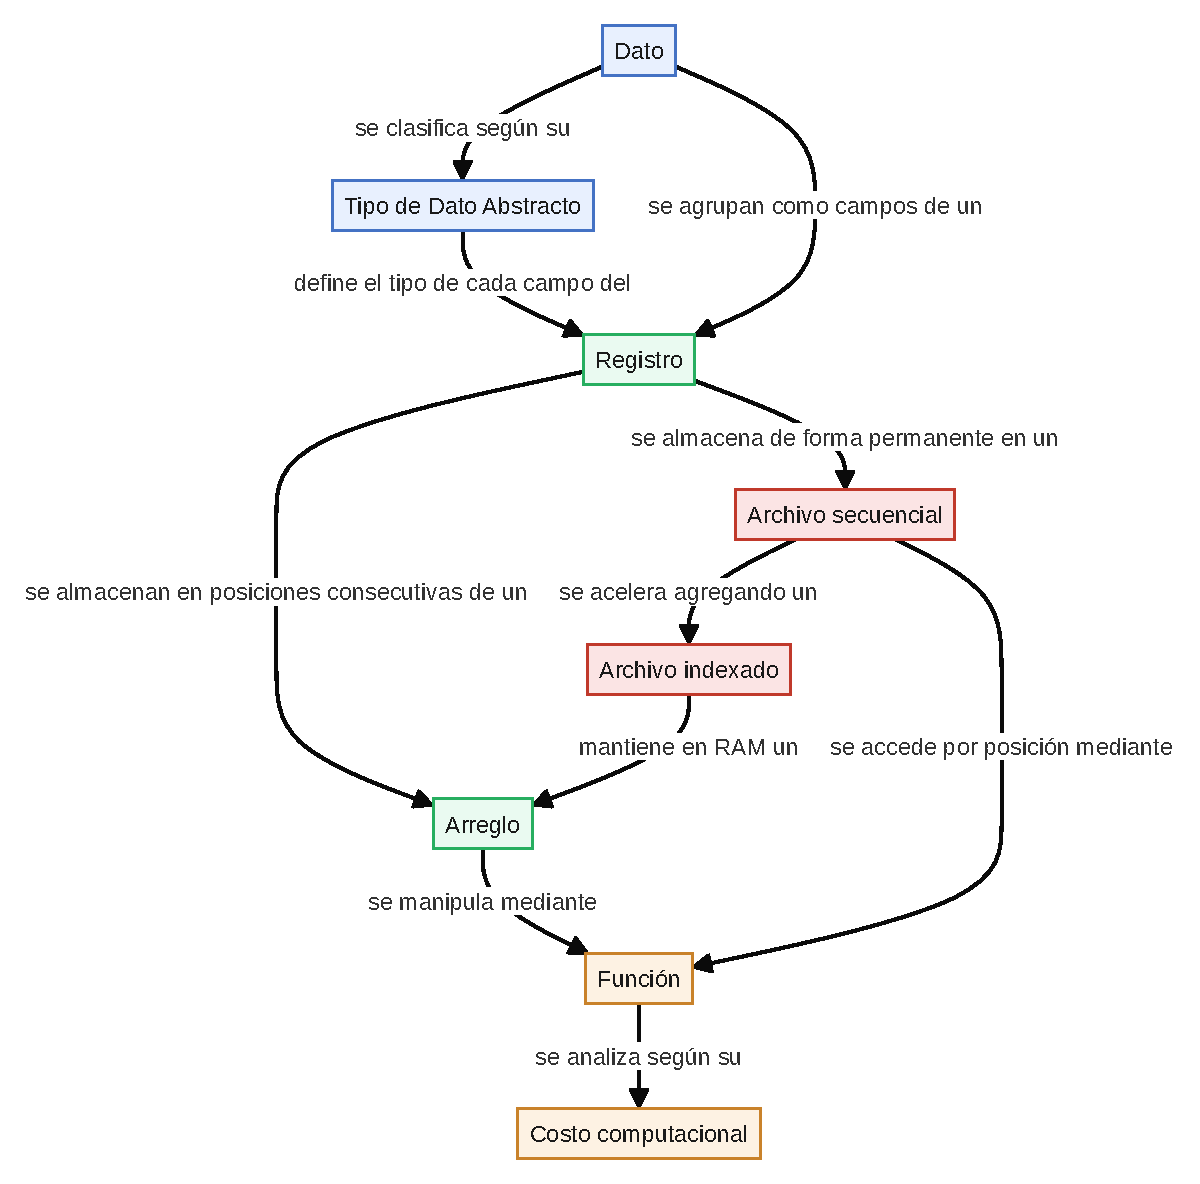
\includegraphics[width=\textwidth]{../diagramas/output/mapa-conceptual.pdf}
    \caption{Mapa conceptual de la investigación}
    \label{fig:mapa-conceptual}
\end{figure}

Un \textbf{Dato} sin clasificar no dice mucho por sí solo: primero se clasifica según su \textbf{Tipo de Dato Abstracto} (entero, cadena, fecha, enumerado), y ese tipo es lo que define cómo se declara cada campo del \textbf{Registro}. Varios registros consecutivos forman un \textbf{Arreglo}, que en este sistema vive tanto en disco (los tres archivos de tamaño fijo) como en RAM (el mapa de posiciones).

Sobre ese arreglo operan las \textbf{Funciones} documentadas en las secciones anteriores, y cada una de ellas se analiza según su \textbf{Costo computacional} en notación Big O, tal como exige el caso de estudio.

Los registros no viven solo en memoria: se guardan de forma permanente en un \textbf{Archivo secuencial}, accesible por posición mediante funciones como \texttt{fseek} y \texttt{fread}. Para no tener que recorrerlo completo en cada búsqueda, ese archivo se acelera agregando un \textbf{Archivo indexado}, que a su vez es justamente el que mantiene en RAM el arreglo (mapa de posiciones) mencionado antes, cerrando el ciclo entre los ocho conceptos.

\newpage
\section{Conclusiones}

El caso de la Universidad XUNA muestra que los problemas administrativos descritos al inicio 
(expedientes duplicados, información inconsistente, búsquedas lentas) no se resuelven simplemente centralizando los datos,
sino decidiendo con cuidado cómo se representan y cómo se accede a ellos. Esa fue la línea que guió todo el diseño propuesto en este informe.

Separar el registro en tres structs, en vez de un bloque único, salió de mirar qué tan seguido cambia cada dato y quién lo usa junto con qué, no de una preferencia de diseño. 

Lo mismo con el mapa de posiciones: no tiene sentido cargar 25\,000 expedientes completos en RAM si alcanza con guardar el carné, la posición en disco y el estado de cada uno.

El patrón ISAM terminó siendo lo que conecta arreglo, archivo secuencial y archivo indexado entre sí: 
la zona ordenada resuelve la búsqueda en $O(\log n)$, 
la lista de recién ingresados evita reordenar el archivo en cada matrícula nueva, 
y el offset calculado a partir del tamaño fijo del registro es lo que permite llegar directo a un registro en disco sin recorrer los demás.

En conjunto, estas decisiones muestran que el diseño de estructuras de datos no depende únicamente de que una solución funcione, 
sino de que su costo computacional se mantenga razonable a medida que la cantidad dato crece. 
Ese es el criterio que se aplicó en cada función documentada a lo largo del informe, y el que deberá mantenerse durante la implementación del sistema en el resto del semestre.


\printbibliography

\end{document}
